\documentclass[11pt,titlepage]{book}
\usepackage{bignotes}
\usepackage{macrosfabbri-basic,macrosfabbri-dg}
%\usepackage[brazil]{babel}  % adequacao para o portugues Brasil
\usepackage[utf8]{inputenc} % Determina a codificacao utiizada

% From Thesis
\newtheorem{assumption}{Assumption}[section]

\usepackage{emptypage}
\usepackage{caption}
\newcommand{\legend}[1]{}
\newcommand{\source}[1]{}
\newcommand{\C}{{\bf C}}
\newcommand{\bpi}{\pi}

\usepackage{epigraph} % for quotes at beginning of chapters etc



\usepackage{colortbl}
\usepackage{booktabs}


% Simplified notation, used for trifocal research at ICERM
% prefix s means ``simplified''
% Basically identical to H&Z with adjustments to take into account constants,
% as well as convenient notation for the normal case of trifocal geometry where
% view 1 is the reference. Also, it must minimize conflict with IJCV'16 /
% Bignotes.

\newcommand{\srot}{\mathtt{R}} % rotation in simplified notation
\newcommand{\stransl}{\mathbf{t}}  % translation vector in simplified notation
\newcommand{\D}{\mathbf{D}} % 3D tangent direction in simplified notation
\newcommand{\dir}{\mathbf{d}} % 2D tangent direction in simplified notation
\newcommand{\li}{\mathbf{l}} % 2D line homog coordinates

\newcommand{\eqr}[1]{$#1$}
\newcommand{\sss}[2]{#1_#2}
\newcommand{\ms}[3]{#1^#2_#3}
\newcommand{\mss}[2]{#1^#2}
\newcommand{\us}[3]{#1^{#2#3}}

\usepackage[usestackEOL]{stackengine}
\usepackage{scalerel}
\parskip \baselineskip
\def\myupbracefill#1{\rotatebox{90}{\stretchto{\{}{#1}}}
\def\rlwd{.5pt}
\newcommand\notate[4][B]{%
  \if B#1\else\def\myupbracefill##1{}\fi%
  \def\useanchorwidth{T}%
  \setbox0=\hbox{$\displaystyle#2$}%
  \def\stackalignment{c}\stackunder[-6pt]{%
    \def\stackalignment{c}\stackunder[-1.5pt]{%
      \stackunder[2pt]{\strut $\displaystyle#2$}{\myupbracefill{\wd0}}}{%
    \textcolor{gray}{\rule{\rlwd}{#3\baselineskip}}}}{%p
      \textcolor{gray}{\strut\kern9pt$\rightarrow$\smash{\rlap{$~\displaystyle#4$}}}}%
}


\includeonly{%
  front-matter,
  intro,
  future,
  todo,
  rotation,
  algebraic-geometry,
  refs,
}

\makenomenclature
\usepackage{bignotes_part2}

\makeindex
\setcounter{tocdepth}{1}

% Redefine the plain page style
\fancypagestyle{plain}{%
\fancyfoot[CE,CO]{\hypersetup{ hidelinks = true, }\textsc{confidential draft, please cite}~\cite[IJCV]{Fabbri:Kimia:IJCV2016}\hypersetup{ hidelinks = false, }}
\fancyfoot[LE,LO,RE,RO]{\thepage}
\renewcommand{\headrulewidth}{0pt}% Line at the header invisible
\fancyhead[RE]{}
\fancyhead[RO]{}
}

\begin{document}

\newpage
%\authorrunning{Fabbri and Kimia}
%\mynewpage
%\listoffigures
%\onehalfspacing
\begin{titlepage}
\begin{center}

 % \vspace*{0.4cm}

 % 
\includegraphics[width=2.5cm, height=2.5cm]{v1.png}
 
\includegraphics[height=1.5cm]{figs/v1.png}
  \vspace{2cm}

%\begin{minipage}[b]{12cm}\noindent
%    \begin{center}
%      {\Large Universidade do Estado do Rio de Janeiro} \\ {\Large
%	Instituto Politécnico - \Large IPRJ}
%    \end{center}
%  \end{minipage}

 % \Large

  %\sffamily

  %\vspace{0.4cm}

\begin{center}
 % {\LARGE \textbf{Método de redução de dimensionalidade não linear: um estudo sobre aplicação de difusão}}
% {\huge \textbf {Um estudo de redução de\vskip1cm
 %  dimensionalidade  por difusão}} \vskip1cm
  {\huge \textbf {Research Notes on Multiview Geometry, Numerical Algebraic
  Geometry, and Machine Learning\\\vskip1em --- Big Notes ---}} \vskip1cm 
 
\end{center}

  \vspace{0.6cm}
  {\LARGE \textbf{Thesis Raw Material Draft}
  }
  \vspace{1em}

%\vspace{5 cm} % eu coloquei este que não tinha
%  \hspace{1cm}\includegraphics[width=0.8\textwidth]{figs/picasso-sketch.png}

\begin{center}
\textbf{Juliana Ventura}\\
\textbf{Advisors: Ricardo Fabbri and Francisco Duarte Moura Neto}
\end{center}

 \begin{center}
  \vspace{0.5 cm}
 
% \usdate
 {\large \textbf{\today}}%\currenttime}}
 \end{center}
\end{center}
\end{titlepage}
\thispagestyle{empty}
\frontmatter

\fancyhead{}
\fancyhead{}
\renewcommand{\headrulewidth}{0pt}% Line at the header invisible
\newpage
 
\pagestyle{fancy}
\fancyhf{}
\fancyfoot[CE,CO]{\hypersetup{ hidelinks = true, }\textsc{confidential draft, please cite}~\cite[IJCV]{Fabbri:Kimia:IJCV2016}\hypersetup{ hidelinks = false, }}
\fancyfoot[LE,LO,RE,RO]{\thepage}

\tableofcontents
%\listoffigures
%\printnomenclature[3.5cm]
\pagestyle{fancy}
\fancyhf{}
\fancyfoot[CE,CO]{\hypersetup{ hidelinks = true, }\textsc{confidential draft, please cite}~\cite[IJCV]{Fabbri:Kimia:IJCV2016}\hypersetup{ hidelinks = false, }}
\fancyfoot[LE,LO,RE,RO]{\thepage}

\chapter{Foreword}

This document contain research notes by Juliana Ventura, Ricardo Fabbri
and Francisco Duarte Moura Neto. 

\section*{How to Cite this Document}
We ask that you at least
cite~\cite{Fabbri:Kimia:IJCV2016,Fabbri:Kimia:Giblin:ECCV12},
as well as other papers from~\url{http://rfabbri.github.io}.

\section*{Disclaimer}
If you gain access to this document, please:
\begin{itemize}
\item Don't blame us for statements that are wrong, this is a \textsc{research
  draft}. Some stuff was written a really long time ago and may not reflect the
  authors' complete and up-to-date knowledge!
\item Intelectual property: this content is partly patented and is property of Brown
  University, Rio de Janeiro State University, FAPERJ/Brazil, CNPq/Brazil, the
  authors, and others. There may be material here that is not permissible to publish at all.
\end{itemize}

\section*{Acknowledgements}
Special thanks to FAPERJ, CNPq and CAPES / Brazil, and ICERM / Brown University.

\mainmatter
\fancyhead[LE]{\nouppercase{\leftmark}}
\fancyhead[RE]{\thepage}
\fancyhead[LO]{\nouppercase{\rightmark}}
\fancyhead[RO]{\thepage}

\newpage
\pagestyle{fancy}
\fancyhf{}
\fancyhead[LE]{\nouppercase{\leftmark}}
\fancyhead[RE]{\thepage}
\fancyhead[LO]{\nouppercase{\rightmark}}
\fancyhead[RO]{\thepage}
\fancyfoot[CE,CO]{\hypersetup{ hidelinks = true, }\textsc{confidential draft, please cite}~\cite[IJCV]{Fabbri:Kimia:IJCV2016}\hypersetup{ hidelinks = false, }}
\fancyfoot[LE,LO,RE,RO]{\thepage}
\mynewpage
\chapter{Introduction}\label{sec:intro}

\subsection{Applications and Broader Impacts}

Computer vision is a branch of Artificial Intelligence concerned with the
understanding of visual information by algorithms running in physical computers.
Within computer vision, the present work is a module that lies at the interface
of computerized photogrammetry, which is the science of extracting objective
measurements from digital images, with higher level AI elements such as
human-inspired levels of flexibility, robustness, semantic and qualitative reasoning. 

The calibration of images taken from multiple views or
video clips and the 3D reconstruction of \emph{general} scenes from these views in a
robust and flexible way, under \emph{uncontrolled acquisition} conditions, are 
paramount goals of computer vision (as opposed to classical photogrammetry),
ambitious even by modern standards.\footnote{Differently than established
literature~\cite{Hartley:Zisserman:book}, we
found it clearer to a wider audience to employ the term `calibration' in the following sense:
\emph{calibration} is a generic term including all types of ``camera estimation'' and ``relative camera geometry estimation'';
intrinsic calibration is what is usually called simply `calibration', \ie, 
estimating intrinsic camera parameters; 
\emph{extrinsic calibration} means estimating the rotational and translational factors
of the camera model,\ie, `pose estimation'; and \emph{full calibration} means both intrinsic
and extrinsic calibration. There are intermediate calibrations as well, \eg, when estimating both the
rotation, translation, and focal length, or estimating relative
camera pose, fundamental matrices or trifocal tensors, in which case only a
subset or variety in the camera parameters are being recovered, which may span across both
intrinsic and extrinsic parameters.}
%
Challenges relate to the large-scale
choices of appropriate representations and techniques to deal simultaneously
with wildly different materials (\eg, non-Lambertian), geometric models (\eg,
general curved manifolds, discontinuities, textures, deformations, at different
scales), region types (\eg, textured and textureless regions), unknown
illumination conditions, shadows and shades, large viewpoint differences,
background clutter, arbitrary number of objects and unknown camera parameters,
to name a few.  
%
Applications include the reconstruction of 3D object models for use in
videogames~\cite{Ablan:3DPhoto:book},
film~\cite{Ablan:3DPhoto:book,Kitagawa:Mocap:book},
archaeology~\cite{Gay:etal:ACVA10,Luhmann:Photogrammetry:book},
architecture~\cite{Luhmann:Photogrammetry:book}, and urban modeling (\eg,
Google Streetview); match-moving in cinematography for mixing virtual content
and real video~\cite{Dobbert:Matchmoving:book}, the organization of a
collection of photographs with respect to a scene (\eg,
Photourisim~\cite{Argarwal:Snavely:etal:ICCV09} and the Look Around feature in
Google Panoramio), robotic manipulation~\cite{Horn:Robot:Vision}, metrology
from cameras in the automobile industry~\cite{Luhmann:Photogrammetry:book}.
Specific cases of more challenging applications of interest to this proposal
have been addressed, such as the reconstruction of the ocean surface in certan
conditions, for monitoring in offshore platforms and ships, as well as for
change detection modulo sea
motion~\cite{Benetazzo:CE2006,Benetazzo:CE2012,Gallego:etal:TGRS201,Fedele:etal:OM2013,Fedele:etal:MCS2012,Benetazzo:etal:CE2016,Gallego:etal:TIP2013,Bergamasco:etal:CG2016,Rapizo:etal:JCR2015,Fabbri:WaterWaves2016,Fabbri:WaterWaves2017,Souza:Fabbri:WaterWaves2017}.

Most existing Structure from Motion and multiview stereo reconstruction methods
suffer from some common problems such as: \emph{(i)} Not being able to bootstrap
calibration from textureless objects; {\em (ii)} Holes in the 3D model
corresponding to homogeneous/reflective/transparent image regions, {\em (iii)}
Oversmoothing of semantically-important details such as ridges, {\em (iv)} Lack
of semantically meaningful surface features, organization and geometric detail;
{\em (v)} Insufficient reliable geometry to model non-rigid scenes.

As prominent Microsoft Research scientist Andrew Fitzgibbon informally put it in
an informal meeting with Fabbri in CVPR 2017, ``in order to 3D-scan a simple mug
using ordinary cameras, we need better techniques''. He has also noted challenges in his image-based
study of the smooth shape of dolphins~\cite{Fitzgibbon:PAMI:dolphincs}. 

While a fully complete working system addressing all the underlying challenges
is beyond current technology, significant progress has been made in the past few
years using approaches that fall into three broad classes, depending on whether
one focuses on correlating isolated points, surface patches, or curvilinear
structures across views, as described below.



\mynewpage
\chapter{Research Directions}\label{sec:future:directions}

Our research is an effort of augmenting Multiple View Geometry to
handle general curved structures, including curves, surfaces and non-rigid phenomena.
The main lines of future research are: the theory and
practice of the multiview differential geometry of surfaces, and
the automatic curve-based calibration of multiple views. A more detailed list of
future work is given below.


\subsection{Theory}
\begin{itemize}
\item Curve-based calibration of 3 views. Research is underway in conjunction with prof.\ Peter Giblin to 
solve the problem of determining trinocular relative pose from
corresponding point-tangents across 3 views. Coupled with our single-view
pose calibration method from Section~\ref{sec:pose:from:curves}, this would allow for complete
curve-based structure from motion systems starting from a set of images 
without any initial calibration. Extending these ideas to include
curvature is another research possibility.
\item Futher study of nonrigid phenomena.
\end{itemize}

\subsection{Practice}
\begin{itemize}
\item Enrichment of the proposed 3D curve sketch with surface patches. 
The 3d curve sketch system is expected to form the initial building block in a broader effort to use
image evidence of the explicit geometry of curves and surfaces and reconstruct
these by integrating information across many views. The 3D curve sketch was
designed to be the initial scaffold on which surfaces may be constructed. It
forms a reliable structure from which to bootstrap a larger
reconstruction system that works under general conditions. One idea for
incorporating surfaces is the use of occlusion relationships to define a rough,
preliminary surface structure between 3D curves. This initial model can
then be optimized for photoconsistency to obtain a more precise surface model.
One way to carry this out is to use a hypothesize-and-test framework, where we
form hypotheses for whether there is a surface patch between two 3D curves, and
test these hypothesis by reprojecting onto views and verifying consistency.
Hypothesis formation could be image-based where we project the 3D curve sketch
onto an image (or a series of reference images), and form region fragments
between neighboring image curves. Each surface hypothesis could be tested by
forming a rough surface model between the underlying 3D curves of the patch
(\eg, a by fitting a minimal surface), and projecting the entire curve sketch
onto another view. Using the model for the surface patch, one can predict what
other curves should be occluded in case the hypothesis is correct. We then look
in the image for any edges that would support the curves that should have been
occluded. If there is support, then the curves are not actually occluded and the
surface hypothesis must be false.  The baisc idea of using image region
fragments has been successful as part of the top-performing 2-view stereo
algorithms in the literature.   
\item Image-based matching of curves in two and three views, so that these
correspondences can be used to bootstrap camera calibration from curves. 
We have done preliminary work using \sift\ descriptors attached to curves, and the
matching results were very promising. The descriptors are rotated to match the
tangent direction of the curve at each sample. There is room for improvement in terms of
efficiency, as we are computing \sift\ descriptors at different scales
for each curve sample, as well as matching all of them. Perhaps
a subsampling strategy should be used, or even a different strategy where the
histogram bins are placed on a global grid built around the entire curve.
\item Extension of the qualitative/geometric ideas of
Appendix~\ref{sec:epipolar} for epipolar geometry to curves. 
\item Development of a better numeric method to measure curvature derivative,
allowing to measure 3D torsion from image curves. Perhaps even a coarse but
robust measurement of curvature derivative could be useful in practice.
\end{itemize}


\mynewpage
\chapter{To Do}\draftnote{Warning: may be obsolete}

\section{Computational Efficiency}
\begin{enumerate}
\item Speedup numerical solvers using machine learning ideas.
\end{enumerate}

\section{Other To-do's}
\begin{itemize}
\item Anything else goes here
\end{itemize}


\mynewpage
\chapter{Rotations}

\section{To Do}

\begin{itemize}
\item Include my lect notes on exp and log and rodrigues from soatto -- GOOD
\item cite this: Metrics for 3D Rotations: Comparison and Analysis JMIV 2009
\end{itemize}


\section{Usual representations of rotation}
We have three majorly used representations: Matrices,
Axis-angle, and Quaternions, as reviewed below.

\section{Matrices}
In terms of roll, pitch, and yaw angles, as in Figure~\ref{fig:yaw:pitch:roll}, the rotation matrix $R = \mathcal M^A_B(id)$ can be decomposed
as $R(\theta,\phi,\psi) =
R_z(\theta)R_y(\phi)R_x(\psi)$, where
\begin{align}
R_z(\theta) &= \begin{bmatrix}
\cos\theta & \sin\theta & 0\\
-\sin\theta & \cos\theta & 0\\
0 & 0 & 1
\end{bmatrix}\\
%
R_y(\phi) &= \begin{bmatrix}
\cos\phi & 0 & -\sin\phi\\
0 & 1 & 0\\
\sin\phi &0 &\cos\phi
\end{bmatrix}\\
%
R_x(\psi) &= \begin{bmatrix}
1 & 0 & 0\\
0 & \cos\psi & \sin\psi\\
0 &-\sin\psi & \cos\psi
\end{bmatrix}
\end{align}

And the form of $R(\theta,\phi,\psi) = R_z(\theta)R_y(\phi)R_x(\psi)$ would be:
\begin{align}
\begin{bmatrix}
\cos\theta\cos\phi & \cos\theta\sin\phi\sin\psi + \sin\theta\cos\psi & 
-\cos\theta\sin\phi\cos\psi + \sin\theta\sin\psi\\
%
-\sin\theta\cos\phi & -\sin\theta\sin\phi\sin\psi + \cos\theta\cos\psi &
\sin\theta\sin\phi\cos\psi + \cos\theta\sin\psi\\
%
\sin\phi & -\cos\phi\sin\psi & \cos\phi\cos\psi
\end{bmatrix}
\end{align}
Note that this is the inverse of the rotation for points while fixing the bases. 
Note also that the order of multiplication of the $x,y,z$ rotation matrices
makes a difference in the final rotation.
\begin{figure}
\centering
   \subfigure[]{ %
    \label{fig:yaw:pitch:roll}
      \begin{minipage}[c]{0.45\linewidth}%
         \centering
        \scalebox{0.4}{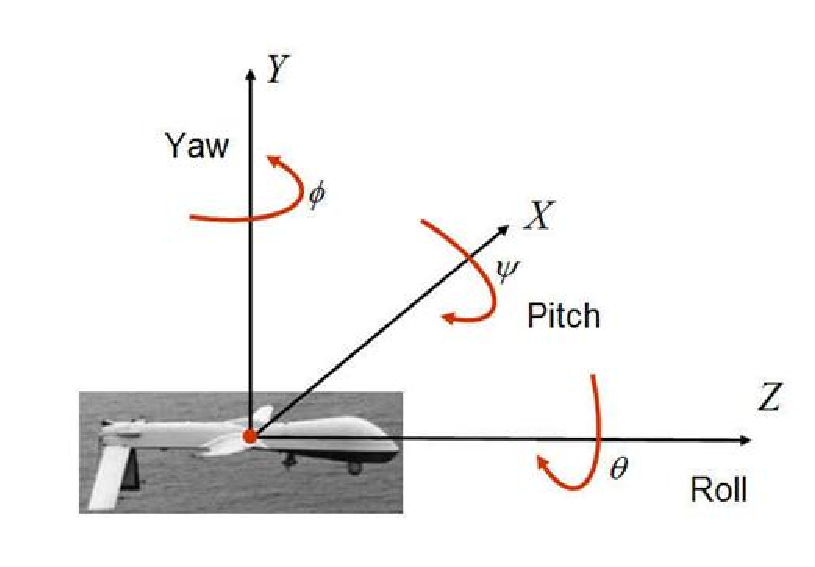
\includegraphics{figs/yaw-pitch-roll.eps}}
      \end{minipage}}
    \subfigure[]{ %
      \label{fig:axis:angle}
      \begin{minipage}[c]{0.45\linewidth}%
         \centering
         \scalebox{0.4}{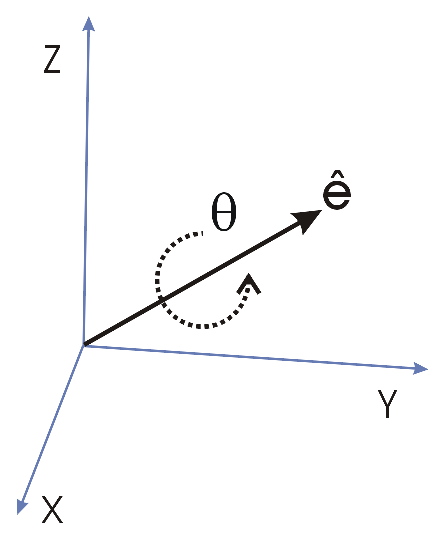
\includegraphics{figs/Euler_AxisAngle.eps}}
      \end{minipage}}
\caption{% 
(a) Orthogonal rotations; (b)
Any 3D rotation can be represented by a rotation of angle $\theta$ around an
axis $\hat{\mathbf{e}}$
}
\end{figure}

\paragraph{Normalization}
When rotation matrices are computed from measured points and camera
observations, it is typical that the resulting rotation matrix does not
satisfy the orthonormal constraints that must hold among the rows and columns.
In order to normalize a 3x3 matrix to insure that it is orthonormal the following operation must be performed:
\begin{equation}\label{eq:r:normalized}
R_{normalized} = R\left[ \left( R^\top R \right)^{\frac{1}{2}}
\right]^{-1}
\end{equation}


\paragraph{Pros}
\begin{itemize}
\item Fastest for rotating large ammounts
of point data, according to~\cite{Schneider:Geometry:book:2003}.
\end{itemize}
\paragraph{Cons}
\begin{itemize}
\item Slower than quaternion for composing rotations
\item Slower than quaternion for normalization that is used due to round-off errors that
occur during optimization. 
\item Problems due to singularities
\item Has 9 parameters (all entries of the $3\times 3$ matrix), even though rotations have 3 degrees of freedom
\end{itemize}

\section{Quaternions}

\todo{I have an improved version with Soatto' insights on $\mathbb C + \mathbb C j$}

The quaternion is a 4-D vector analogous to the complex number. Rotations can be represented as unit
quaternions. In order to define product of quaternions, its 4 parameters
are grouped into a 3D vector part and a scalar part along with an associated algebra:
\begin{align}
q &= q_0 + \mathbf q = q_0 + iq_1 + jq_2 + kq_3
\intertext{Where $i,j,k$, the hypercomplex numbers, play a similar role to the imaginary axis in complex
numbers. The conjugate of a quaternion is defined as:}
q^* &= q_0 - \mathbf q
\shortintertext{Its magnitude is:}
|q| &= qq^* = (q_0 + \mathbf q)(q_0 - \mathbf q) = q_0^2 - \mathbf q\mathbf q
\end{align}
The meaning of $\mathbf q\mathbf q$ comes from the axioms for multiplying the
$i,j,k$ components:
\begin{align}
i^2 &= j^2 = k^2 = -1\\
ij &= k,\,\, ji = -k\\
jk &= i,\,\, kj = -i\\
ki &= j,\,\, ik = -j
\end{align}
In order to multiply quaternions, just use usual distributive laws, being careful
with the order, and applying the above axioms. The meaning of multiplication is
more clear if we first consider the product of two different quaternion vectors:
\begin{align}
&\mathbf p\mathbf q = (ip_1 + jp_2 + kp_3)(iq_1 + jq_2 + kq_3) =\notag\\
&i(p_2q_3 - p_3q_2) + j(p_3q_1 - p_2 q_3) + k(p_1q_2 - p_2q_1) - (p_1q_1 + p_2q_2
+ p_3q_3) = \notag\\
&\mathbf p\times\mathbf q - \mathbf p\cdot \mathbf q
\end{align}
It follows that 
\begin{align}
\mathbf q\mathbf q &= \mathbf q\times\mathbf q - \mathbf q\cdot\mathbf q =
-(q_1^2 + q_2^2 + q_3^2)
\shortintertext{so:}
qq^* &= (q_0^2 + q_1^2 + q_2^2 + q_3^2) = |q|^2
\end{align}
which is a reasonable interpretation of a conjugate operation.
The inverse of a quaternion is:
\begin{equation}
\mathbf q^{-1} = \frac{q^*}{|q|^2}
\end{equation}
The rotation about a unit vector $\hat{\mathbf e}$ is:
\begin{equation}
q = \cos \frac{\theta}{2} + \sin \frac{\theta}{2}\hat {\mathbf e}
\end{equation}
Note that $|q| = 1$. We can encode a regular 3-vector $\Gama$ as a
quaternion as $\Gamma = 0 + \Gama$. The rotation of this vector is defined as:
\begin{equation}
\Gamma' = q\Gamma q^*
\end{equation}

\paragraph{Example.} 
To illustrate consider a point in the $x-y$ plane which is on the $x$ axis,
$\Gama = (2,0,0)$. Rotate the point around the z axis by 90 degrees. The
rotation is expressed as:
\begin{equation}
q = \cos 45^\circ + \sin 45^\circ (0i + 0j + k) = 0.707 + 0.707k
\end{equation}
The rotation of $\Gama$ is:
\begin{equation}
\Gamma' = (0.707 + 0.707k)(0 + 2i)(0.707 - 0.707k) = 0 + 0i + j + 0k
\end{equation}
which is a vector along the $y$ axis, as expected.

Composing two rotations $p$ and $q$ is just the product, so that:
\begin{equation}
\Gamma' = (pq)\Gamma(pq)^*
\end{equation}

\paragraph{Quaternion to Rotation Matrix}
\begin{equation}\label{eq:quaternion:to:rotation:matrix}
q\Gamma q^* \rightarrow
\begin{bmatrix}
q_0^2 + q_1^2 - q_2^2 - q_3^2 & 2(q_1q_2 - q_0q_3) & 2(q_1q_3 + q_0q_2)\\
2(q_1q_2+q_0q_3) & q_0^2 - q_1^2 + q_2^2 - q_3^2 & 2(q_2q_3 - q_0q_1)\\
2(q_1q_3 - q_0q_2) & 2(q_2q_3 + q_0q_1) & q_0^2 - q_1^2 -q_2^2 + q_3^2
\end{bmatrix}
\Gama,
\end{equation}
with $q_0^2 + q_1^2 + q_2^2 + q_3^2 = 1$.

\paragraph{Rotation Matrix to Quaternion}
\begin{equation}
R = 
\begin{bmatrix}
r_{00} & r_{01} & r_{02}\\
r_{10} & r_{11} & r_{12}\\
r_{20} & r_{21} & r_{22}
\end{bmatrix}
\end{equation}
\begin{equation}
q_0 = \frac{1}{2}\sqrt{r_{00}^2 + r_{11}^2 + r_{22}^2},\,\,
q_1 = \frac{r_{21} - r_{12}}{4q_0},\,\,
q_2 = \frac{r_{02} - r_{20}}{4q_0},\,\,
q_3 = \frac{r_{10} - r_{01}}{4q_0}
\end{equation}

\paragraph{Axis-angle to Quaternion}
As noted above, the rotation about a unit vector $\hat{\mathbf e}$ is:
\begin{equation}
q = \cos \frac{\theta}{2} + \sin \frac{\theta}{2}\hat {\mathbf e}
\end{equation}
Note that $|q| = 1$. 

\paragraph{Normalization}
In order to normalize a quaternion to be unit, we simply do:
\begin{equation}
q_{normalized} = \frac{qq^*}{|q|^2}
\end{equation}
Compared to~\eqref{eq:r:normalized}, this is a lot cheaper.


\paragraph{Pros}
\begin{itemize}
\item Said do be the best for optimization. Vxl uses it, Faugeras uses it.
\draftnote{TODO: clarify}
\item Useful to give solvable algebraic equations involving rotations, by
using~\ref{eq:quaternion:to:rotation:matrix}.  Astr\"om~\cite{Astrom:etal:Polysolver:IJCV09} uses it. 
\item Easy to compose through multiplication. Faster than matrices for this.
\item Normalization is very fast compared to matrices
\item No singularity in the parametrization
\end{itemize}

\paragraph{Cons}
\begin{itemize}
\item Slower than rotation matrices for transforming points. However, difference
is negligible for large number of points.
\draftnote{todo: quantify}
\item 4 parameters for the 3 degrees of freedom of rotation matrices
\end{itemize}

\paragraph{Research directions}
Study quaternions in:
\begin{itemize}
\item Penrose's ``The Road to Reality'' book has a good chapter on quaternions,
clifford and grassman algebras.
\item Wikipedia about quarternions and rotations.
\item Book on rotations, quaternions and double groups
\item (Vague): Recall that Stolfi's oriented projective geometry has more to do with
rotation geometry.
\end{itemize}

\section{Axis-Angle}

We can represent any 3D rotation by a rotation around a rotation axis
$\hat{\mathbf e}$ and angle $\theta$. This can be encoded as $\mathbf e =
\theta\cdot\hat{\mathbf e}$, i.e.\ a vector whose direction is the axis of
rotation, and the magintude is the angle of rotation around such axis.

\paragraph{Axis-Angle to Rotation Matrices}

To convert from the axis-angle to a rotation matrix, we use the Rodrigues
formula~\cite{Ma:Soatto:etal:book}:

\begin{equation}\label{eq:rodrigues:rotation:formula}
R(\theta,\hat{\mathbf e}) = I + \frac{\sin\theta}{\theta} \hat{\mathbf e}_\times
+ \frac{(1 - \cos\theta)}{\theta^2}\hat{\mathbf e}_\times^2
\end{equation}
where
\begin{align}
\hat{\mathbf e} &= 
\left[ a\,\,b\,\,c \right]^\top\\
\hat{\mathbf e}_\times&= \left[\begin{array}{ccc} 0 & -c & b\\ c & 0 & -a\\ -b &
a & 0 \end{array} \right]
\end{align}

\paragraph{Rotation Matrices to Axis-Angle.}
Eigen-decomposition of the rotation matrix yields the eigenvalues $1$, and $\cos\theta \pm i\sin\theta$.
The Euler axis is the eigenvector corresponding to the eigenvalue of $1$, and the $\theta$ can be computed from the remaining eigenvalues.


\paragraph{Pros}
\begin{itemize}
\item Due to the Rodrigues formula, it seems easy to use this representation in
equations
\end{itemize}

\paragraph{Cons}
\begin{itemize}
\item Hard to compose two transformations
\item Prone to singularities
\end{itemize}

\section{Exponential maps}

TODO: merge in notes from Taubin, Ma's book, and other sources.

\section{Cayley Rational Parametrization}
TODO: merge in notes from Taubin

\section{Estimating Rotations}
Rotations and rigid motions in general can be estimated from noisy 3D-3D point
correspondences using procrustes analysis (see e.g.\ Matlab's procrustes
function in the statistics toolbox). Minimal problems involving rotation seem hard to
solve. These problems can be found in inverse kinematics in robotics books. See
Horn's robotics book or Paul's book from MIT press, or even a chapter
in~\cite{Cox:etal:Ideals}. The state-of-the-art techniques for robustly estimating models
that involve rotation is, to the best of our knowledge, Kalle Astr\"om's
work~\cite{Astrom:etal:Polysolver:IJCV09} on minimal solvers together with
RANSAC.  

Here is a practical way of estimating a rotation matrix in Matlab, given 4
known vectors transformed to other 4 known vectors:
\begin{verbatim}
%
% Generate a random rotation matrix
%
[Q dummy]= qr(rand(3));
Q

%
% Random 4 vectors in R^3 in the first coordinate
%
A=randn(3,4);
B=Q*A; % Coordinates in the second system

%
% Estimates Q from A and B
%
Qest = B/A

%
% Do this if you don't trust your data and
% want to reorrthogonalize Qest
%
[U,S,V]=svd(Qest);
Qest = U*V'
\end{verbatim}

Here is a way of estimating using procrustes:
\begin{verbatim}
 >> A = randn(4,3); % four random vectors in 3-D
 >> [U,S,V] = svd(randn(3)); T = U*V'; % random orthogonal matrix
 >> T
T =
      -0.91586 -0.14665 -0.37375
      0.084785 0.83926 -0.53707
       0.39244 -0.52357 -0.75621
 >> B = A*T; % rotate A
 >>
 >> [d,B1,tr] = procrustes(B,A);
 >> tr.T % rotation component: same as original T
ans =
      -0.91586 -0.14665 -0.37375
      0.084785 0.83926 -0.53707
       0.39244 -0.52357 -0.75621
 >> tr.c % translation component: 0
ans =
    2.2204e-16 5.5511e-17 0
    2.2204e-16 5.5511e-17 0
    2.2204e-16 5.5511e-17 0
    2.2204e-16 5.5511e-17 0
 >> tr.b % scale component: 1
ans =
             1
\end{verbatim}

Question: is 4 vectors the minimum needed to get $\rot$?

\subsection{Rotation minimizing turning angle}

Given unit vectors $\vec v$ and $\vec w$, we can use Rodrigues'
formula~\eqref{eq:rodrigues:rotation:formula} to compute the rotation that
minimizes the turning angle amongst all the rotations that take $\vec v$ to
$\vec w$. We just write
\begin{equation}
\rot(\theta,\hat{\mathbf e}) = I + \sqrt{1 - (\vec v^\top\vec w)^2}\hat{\mathbf e}_\times
+ \vec v^\top\vec w\hat{\mathbf e}_\times^2,
\end{equation}
with $\hat \e = \frac{\vec v \times \vec w}{\sqrt{1 - (\vec v^\top\vec w)^2}}$.
If $\vec v =  \vec w$, we simply define the minimal rotation to be the identity
matrix. If $\vec v =  -\vec w$ we have a singularity in the
$\rot(\theta,\hat{\mathbf e})$ function.

%\include{projective-geometry}
\mynewpage
\chapter{Algebraic Geometry}\label{sec:algebraic:geometry}

\indraftnote{Some of this material goes into the main book. Here we're just
putting all our notes in}

\indraftnote{This is getting into shape but is waaay behind what we have in other documents.}

\section{Computational Aspects}

\section{David Pinho's MSc.\ Notes}
Esta seção se destina a apresentar um resumo das definições básicas em Geometria Algébrica, bem como alguns conceitos e definições mais avançados necessários ao entendimento do procedimento de solução de sistemas de equações polinomiais. Para acessar um detalhamento maior da teoria juntamente com as demonstrações dos teoremas, o leitor pode consultar os livros Cox et al. (2005) e Cox et al. (2007).

\subsection{Definições básicas}

A Geometria Algébrica tem como objetivo principal de estudos as variedades algébricas, os objetos geométricos
formados pelos pontos que são soluções de um sistema de equações polinomiais. Para realizar esse estudo, utiliza técnicas de álgebra comutativa em conjunto com a linguagem geométrica.

{\it Monômios} são o produto de $n$ variáveis da forma $x_1^{\alpha_1}\cdot x_2^{\alpha_2} \cdot ... \cdot x_n^{\alpha_n}$ onde os expoentes são números inteiros não-negativos. O grau total de um monômio é a soma dos expoentes das variáveis e é denotado por $|\alpha|=\alpha_1+\alpha_2+...+\alpha_n$, e para simplificar a notação é adotada a convenção onde $\alpha=(\alpha_1,\alpha_2,...,\alpha_n)$ é o vetor dos expoentes e $x^\alpha=x_1^{\alpha_1}\cdot x_2^{\alpha_2} \cdot ... \cdot x_n^{\alpha_n}$ é a representação do monômio.

{\it Polinômios} são combinações lineares dos monômios denotados por
\begin{equation*}
f=\sum_\alpha a_\alpha x^\alpha,\quad\text{onde}\quad a_\alpha\in k.
\end{equation*} 
Os coeficientes desses polinômios pertencem a um conjunto numérico denominado {\it corpo}, denotado por $k$, que pode ser o conjunto dos números complexos ou reais, por exemplo. Informalmente, corpo é um conjunto fechado para adição, subtração, multiplicação e divisão com suas propriedades usuais. O conjunto de todos os polinômios nas $n$ variáveis definidas num corpo $k$ é denotado por $k[x_1,...,x_n]$.

Se estivermos trabalhando com pouca variáveis podemos utilizar $x$, $y$ e $z$ e como exemplo temos
\begin{equation*}
f=2x^3y^2z+\frac{2}{3}y^3z^3-3xyz+y^2\quad\in\quad\mathbb{Q}[x,y,z],
\end{equation*} 
onde
\begin{itemize}
\item os {\it coeficientes} são 2, $\frac{2}{3}$, -3 e 1,
\item os {\it termos} são cada monômio junto com o respectivo coeficiente
\item o {\it grau total} do polinômio é o grau do monômio de maior grau; no caso temos dois monômios com grau 6.
\end{itemize}

A soma e o produto de dois polinômios também são polinômios, mas um polinômio $f$ divide um polinômio $g$ apenas se existe um polinômio $h$ onde $g=f\,h$. Assim, entre polinômios ficam satisfeitos os axiomas de adição e multiplicação em um corpo, mas não a existência de um inverso multiplicativo, pois por exemplo, $f=\frac{1}{x}$ não é um polinômio. Os elementos que obedecem essa estrutura formam um {\it anel comutativo}, com estudos feitos com base na {\it álgebra comutativa}, e por isso o conjunto $k[x_1,...,x_n]$ é chamado {\it anel de polinômios}.

\subsection{Ideal e variedade}
Um espaço $n$-dimensional num corpo $k$ é definido como
\begin{equation*}
k^n=\{(a_1,...,a_n)\,/\, a_1,...,a_n\in k\},
\end{equation*}
e é possível relacionar polinômios com um espaço $n$-dimensional observando que um polinômio nos dá uma função
\begin{equation*}
f:k^n\rightarrow k\quad\text{com}\quad f=\sum_\alpha a_\alpha x^\alpha\quad \in\quad k[x_1,...,x_n].
\end{equation*}
A capacidade em tratar polinômios como funções é o que possibilita ligar álgebra e geometria através das chamadas {\it variedades}, definida a seguir e denotada por ${\bf V}$.
\begin{equation*}
{\bf V}(f_1,...,f_s)=\{(a_1,...,a_n)\in k^n/\, f_i(a_1,...,a_n)=0, \,\forall\,\, 1\le i\le s\}.
\end{equation*}
Portanto, variedades podem ser entendidas como o conjunto de vetores que são solução de um sistema de equações polinomiais, e que fornecem uma representação geométrica para a solução do sistema sempre que possível.

Como exemplo, temos na Figura \ref{fig.variedades} a representação geométrica das variedades ${\bf V}(xy-x^3+1)$ e ${\bf V}(-x^2-y+z)$, onde cada ponto no plano e no espaço é representado pelas soluções de $xy-x^3+1=0$ e $-x^2-y+z=0$, respectivamente.
\begin{figure}
\caption{Variedades.}
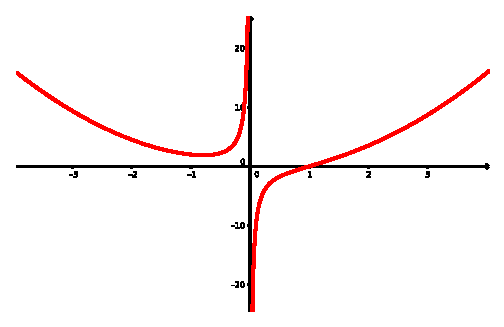
\includegraphics[width=.57\hsize]{figs/variedade-1}\hfill
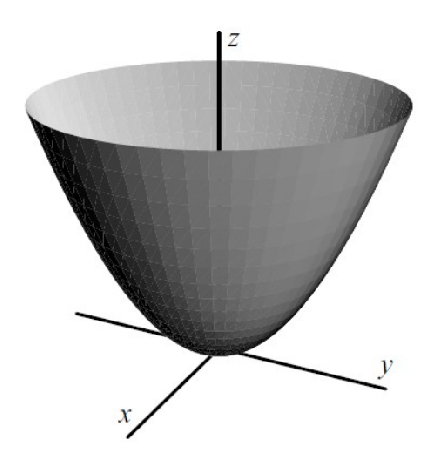
\includegraphics[width=.4\hsize]{figs/variedade-3D}\hfill
\legend{As representações geométricas podem ser obtidas usando as funções ({\tt a}) $y=\frac{x^3-1}{x}$ e ({\tt b}) $z=x^2+y$.}
\source{({\tt a}) O autor. ({\tt b}) Cox et al. (2005).}
\label{fig.variedades}
\end{figure} 

{\it Ideal} é um subconjunto de $k[x_1,...,x_n]$ denotado por $I$ que satisfaz as condições:
\begin{itemize}
\item $0\in I$;
\item $f,g\,\in I \Rightarrow (f+g)\in I$;
\item $f \in I$ e $h \in k[x_1,...,x_n] \Rightarrow h\,f \in I$. 
\end{itemize}

Se $f_1,...,f_s$ são polinômios em $k[x_1,...,x_n]$ então podemos definir um ideal através desses polinômios que são chamados de {\it base} do ideal, usando a notação
\begin{equation*}
I=\left\langle f_1,...,f_s \right\rangle = \{\sum_{i=1}^s h_if_i\,:\,h_1,...,h_s \in k[x_1,...,x_n]\}.
\end{equation*}
Por exemplo, para sabermos se o polinômio $x^2-2x+2-y$ pertence ao ideal $\left\langle x-1-t\,,\,y-1-t^2 \right\rangle$ devemos verificar se é possível escrevê-lo como combinação das bases desse ideal, 
\begin{equation*}
x^2-2x+2-y=(x-1+t)(x-1-t)+(-1)(y-1-t^2).
\end{equation*}
Um mesmo ideal pode ser formado por bases diferentes e, quando isso acontece, as variedades definidas por cada base também são iguais, ou seja
\begin{equation*}
\left\langle f_1,...,f_s \right\rangle = \left\langle g_1,...,g_s \right\rangle \Rightarrow {\bf V}(f_1,...,f_s)={\bf V}(g_1,...,g_s).
\end{equation*}
Por exemplo, temos a seguir um ideal formado por bases diferentes (podemos verificar que se trata do mesmo ideal escrevendo os polinômios da esquerda como combinação dos polinômios da direita e reciprocamente) e que possuem variedades iguais:
\begin{equation*}
\left\langle 2x^2+3y^2-11\,,\,x^2-y^2-3 \right\rangle = \left\langle x^2-4\,,\,y^2-1 \right\rangle,\,\, \text{logo}
\end{equation*}
\begin{equation}\label{eq.variedades}
{\bf V}(2x^2+3y^2-11\,,\,x^2-y^2-3)={\bf V}(x^2-4\,,\,y^2-1)=\{(\pm2,\pm1)\}.
\end{equation}
Observe que todos os polinômios de um ideal terão o mesmo conjunto variedade gerado pelos polinômios da base. Observe ainda, que a base de um ideal pode ser pensada como um sistema de equações polinomiais, e que para encontrarmos o conjunto solução do sistema (variedade) podemos converter a base dada numa base mais simples conforme a relação \ref{eq.variedades}. Mais à frente veremos que é exatamente esse o procedimento realizado pelas bases de Gr\"obner.

\subsection{As bases de Gr\"obner}

Para sabermos se um polinômio $f$ pertence a um ideal devemos dividir $f$ pelas bases do ideal e verificar se o resto é zero, pois assim $f$ pode ser escrito como combinação dos polinômios da base. Na divisão de polinômios de uma variável o resto é único, mas para polinômios de mais de uma variável, tanto o resto como os quocientes podem variar dependendo da ordem dos divisores e da ordenação de monômios escolhida ({\it lexicográfica, lexicográfica graduada e lexicográfica graduada reversa}). Para detalhes sobre divisão de polinômios de várias variáveis consultar Cox et al. (2005). 

Por exemplo, vamos verificar se o polinômio $f=xy^2-x$ pertence ao ideal $I=\left\langle xy+1\,,\,y^2-1 \right\rangle$. Efetuando a divisão de $f$ por $\{xy+1\,,\,y^2-1\}$ nesta ordem, obtemos
\begin{equation*}
xy^2-x=y(xy+1)+0(y^2-1)+(-x-y)
\end{equation*}  
com resto $-x-y$. Mas efetuando a divisão na ordem $\{y^2-1\,,\,xy+1\}$ teremos
\begin{equation*}
xy^2-x=x(y^2-1)+0(xy+1)+0
\end{equation*} 
com resto zero. Assim, $f\in I$ e vemos que, dada uma base qualquer de $I$, o resto zero é uma condição suficiente para que $f\in I$ mas não é uma condição necessária. 

Precisamos de uma base que facilite verificar se um polinômio pertence a um ideal, e as bases de Gr\"obner tem essa propriedade, pois um polinômio $f$ quando dividido pelas bases de Gr\"obner deixa resto único, não importanto a ordem dos divisores (base do ideal). Assim, sendo $G=\{g_1,...,g_t\}$ uma base de Gr\"obner, então 
\begin{equation*}
f\in I \Leftrightarrow \text{o resto da divisão de $f$ por $G$ é zero}.
\end{equation*}
Essa propriedade é tão importante que às vezes é tomada como a própria definição para as bases de Gr\"obner. O resto da divisão de um polinômio $f$ por $G=\{g_1,...,g_t\}$ é denotado por $\overline{f}^G$. Por exemplo, dividindo $f=x^5y$ por $G=\{x^2y-y^2\,,\,x^4y^2-y^2\}$ é $\overline{x^5y}^G=xy^3$, pois
\begin{equation*}
x^5y=(x^3+xy)(x^2y-y^2)+(0)(x^4y^2-y^2)+xy^3.
\end{equation*}
Para verificarmos se uma base é uma base de Gr\"obner utilizamos o {\it critério de Buchberger}, e caso não seja, toda base de um ideal pode ser convertida numa base de Gr\"obner utilizando o {\it algoritmo de Buchberger}. 

\subsection{Resolvendo sistemas com as bases de Gr\"obner}

Considere o sistema
\begin{empheq}[left=\empheqlbrace]{align*}
x^2+y^2+z^2&=1\\
x^2+z^2-y&=0\\
x-z&=0,
\end{empheq}
cujas soluções podem ser obtidas como a extração do conjunto variedade do ideal
\begin{equation*}
I=\left\langle x^2+y^2+z^2-1\,,\,x^2+z^2-y\,,\,x-z\right\rangle. 
\end{equation*}
Como toda base de um ideal pode ser convertida numa base de Gr\"obner, aplicando o algoritmo de Buchberger calculamos uma nova base para o ideal
\begin{equation*}
I=\left\langle x-z\,,\,-y+2z^2\,,\,z^4+\frac{1}{2}z^2-\frac{1}{4}\right\rangle. 
\end{equation*}
Como um ideal com bases diferentes possui o mesmo conjunto variedade, podemos converter as bases de Gr\"obner num novo sistema que terá o mesmo conjunto solução do anterior,
\begin{empheq}[left=\empheqlbrace]{align*}
x-z&=0\\
-y+2z^2&=0\\
z^4+\frac{1}{2}z^2&=\frac{1}{4}.
\end{empheq}
Note que a última equação do sistema depende apenas de uma variável, que pode ser obtida através de um método numérico. O {\it teorema da eliminação} garante que, definida uma ordenação de monômios, as variáveis de um sistema são eliminadas de acordo com a precedência dessa ordem. Depois de calculada a primeira variável, por retro-substituição podemos determinar o valor das variáveis restantes, onde tal retro-substituição é garantida, sob determinadas condições, pelo {\it teorema da extensão}. Alguns softwares de computação algébrica (como Maple) possuem pacotes para computação das bases de Gr\"obner. O procedimento apresentado aqui para solução de sistemas possui algumas deficiências que serão comparadas com o procedimento a seguir no final do apêndice.

\subsection{Álgebra de um espaço dimensional finito}

Na divisão de um polinômio $f\in k[x_1,...,x_n]$ por uma base de Gr\"obner $G$ obtemos a expansão
\begin{equation*}
f=h_1g_1+...+h_tg_t+\overline{f}^G,
\end{equation*} 
onde $\overline{f}^G$ é uma combinação de monômios que não são divisíveis pelos termos líderes dos polinômios de $G$. Mas existem outros polinômios em $k[x_1,...,x_n]$ que deixam o mesmo resto que $f$ na divisão por $G$. Assim $f$ definde uma {\it classe de equivalência} dada por
\begin{equation*}
[f]=\{p\in k[x_1,...,x_n]\,/\,p\equiv f\, \text{mod}\, I\}.
\end{equation*}
Ou seja, assim como temos os polinômios que pertencem ao ideal $I$, temos também o conjunto dos polinômios que não pertencem ao ideal, e cada um desses polinômios pertence à sua classe de equivalência. O conjunto de todas as classes de equivalência de um ideal forma um anel denominado {\it anel quociente}, denotado por
\begin{equation*}
k[x_1,...,x_n]/I=\{[f]\,/\,f\in k[x_1,...,x_n]\}.
\end{equation*}

Quando multiplicamos dois restos de um ideal, $\overline{f}^G\cdot\overline{p}^G$, podemos obter um polinômio que pertence ao ideal, mas quando somamos dois restos ou multiplicamos um resto por um escalar, o polinômio gerado continua pertencendo ao anel quociente $k[x_1,...,x_n]/I$. Por essa e outras características, temos que esse anel tem a estrutura de um {\it espaço vetorial} e é denominado {\it Álgebra}. Os monômios que não são divisíveis pelos termos líderes de $G$ formam uma base para essa Álgebra, denominada {\it base linear}. Considere como exemplo o ideal gerado por 
\begin{equation}\label{eq.base-G}
G=\{x^2+\frac{3xy}{2}+\frac{y^2}{2}-\frac{3x}{2}-\frac{3y}{2}\,,\,xy^2-x\,,\,y^3-y\},
\end{equation}
cujo polinômios têm os termos líderes dados por $\{x^2\,,\,xy^2\,,\,y^3\}$. Extraindo os monômios que não são divisíveis pelos termos líderes formamos a base linear
\begin{equation*}
B=\{1\,,\,x\,,\,y\,,\,xy\,,\,y^2\},
\end{equation*}
onde os cinco monômios são uma base do espaço vetorial para a álgebra $A={\mathbb C}[x,y]/I$. Assim, todo polinômio que não pertence a $I$ pode ser escrito como uma {\it combinação linear} dos monômios de $B$.

A base linear $B$ tem dimensão finita e sempre terá desde que sejam satisfeitas as condições do {\it teorema da finitude}, para o qual a principal condição é que sendo $G$ uma base de Gr\"obner para um ideal $I \subset k[x_1,...,x_n]$, então para cada $1\le i\le n$, existe um $m_i\ge 0$ tal que $x_i^{m_i}$ é o termo líder de algum $g\in G$. Ou seja, considerando a base $G$ na relação \ref{eq.base-G}, se por exemplo $y^{m_y}$ não pertencesse ao conjunto dos termos líderes para algum $m_y$, não teríamos um expoente que pudesse restringir $y$ a pertencer à base $B$, e esta seria infinita.

\subsection{Resolvendo sistemas com autovalores e autovetores}

A ideia principal é explorar a estrutura de $A=k[x_1,...,x_n]/I$ para estimar o valor de alguma funcão $f$ nos valores de $V$. Observe que nossa tarefa é encontrar os valores de $x_i\in (x_1,...,x_n)$ onde $(x_1,...,x_n)\in V$, assim podemos tomar a função $f=x_i$, pois estimar o valor para $f$ cumprirá a tarefa de encontrar os valores de cada componente do vetor solução.

Para determinar o valor de cada variável é definido um operador linear $m_{x_i}$ como a multiplicação de cada variável $x_i$ pelos polinômios $b$ da base $B$.
\begin{equation*}
m_{x_i}:A\rightarrow A\quad\text{onde}\quad m_{x_i}([b])=x_i\cdot[b].
\end{equation*} 
Desta forma, os possíveis valores para a variável $x_i$ são computados através da decomposição em autovalores da matriz $m_{x_i}$. Por definição em Álgebra Linear, para encontrarmos a matriz $m_{x_i}$,  devemos expandir $p_j=x_i\cdot b_j$ em termos da base $B$, e tomar a transposta da matriz dos coeficientes dessa expansão.

Contudo, multiplicando dois elementos de $A$, não podemos garantir que o resultado $p_j$ seja um elemento de $A$ que possa ser escrito como combinação linear dos elementos de $B$. Assim, devemos escrever a expansão de $p_j$ em termos dos elementos da base $G$ para obter o resto $\overline{p}^{G}$. Como todo polinômio
\begin{equation}\label{eq.resto-mod}
p\equiv\overline{p}^{G}\,\text{mod}\,I,
\end{equation} 
podemos expandir $\overline{p}^{G}$ ao invés de $p$. 

Como exemplo, vamos calcular as soluções do sistema formado pelos polinômios da base $G$ em \ref{eq.base-G},
\begin{empheq}[left=\empheqlbrace]{align*}
x^2+\frac{3xy}{2}+\frac{y^2}{2}-\frac{3x}{2}-\frac{3y}{2}&=0\\
xy^2-x&=0\\
y^3-y&=0,
\end{empheq}
com termos lideres $\{x^2\,,\,xy^2\,,\,y^3\}$ e base $B=\{1\,,\,x\,,\,y\,,\,xy\,,\,y^2\}$. Determinando primeiramente os valores para $x$ temos que $m_x(b_j)=x\cdot b_j$, portanto
\begin{equation*}
\begin{array}{rcccl}
x\cdot1 &= &x& = &0 \cdot 1 + 1 \cdot x + 0 \cdot y + 0 \cdot xy + 0 \cdot y^2\\\\
x \cdot x &= &x^2&=& 0 \cdot 1 + \frac{3}{2} \cdot x + \frac{3}{2} \cdot y - \frac{3}{2} \cdot xy\, - \,\frac{1}{2} \cdot y^2\\\\
x \cdot y &=& xy &= &0 \cdot 1 + 0 \cdot x + 0 \cdot y + 1 \cdot xy + 0 \cdot y^2\\\\
x \cdot xy &=& x^2y &= &0 \cdot 1\, - \,\frac{3}{2} \cdot x \,-\, \frac{1}{2} \cdot y + \frac{3}{2} \cdot xy + \frac{3}{2} \cdot y^2\\\\
x \cdot y^2 &= &xy^2& =& 0 \cdot 1 + 1 \cdot x + 0 \cdot y + 0 \cdot xy + 0 \cdot y^2.
\end{array}
\end{equation*}
Tomando a transposta dos coeficientes temos a denominada {\it matriz de ação},
\begin{equation*}
m_x=
\begin{bmatrix}
0&0&0&0&0\\\\
1&\frac{3}{2}&0&-\frac{3}{2}&1\\\\
0&\frac{3}{2}&0&-\frac{1}{2}&0\\\\
0&-\frac{3}{2}&1&\frac{3}{2}&0\\\\
0&-\frac{1}{2}&0&\frac{3}{2}&0
\end{bmatrix},
\end{equation*}
e os valores para $x$ são dados pelos autovalores $\{-1,2,1,1,0\}$, que podem ser calculados usando o método em \ref{sec.potencias-autovalores}.
 De forma análoga, podemos determinar os valores de $y$ através dos autovalores $\{1,-1,1,-1,0\}$ de $m_y$. As soluções do sistema é o conjunto variedade do ideal $I$ que tem como base $G$,
 \begin{equation*}
 V(I)=\{(-1,1),(2,-1),(1,1),(1,-1),(0,0)\}.
 \end{equation*}

Podemos ver que na expansão de $x\cdot b_j$ acima, os monômios $\{x^2\,,\,x^2y\,,\,xy^2\}$ não podem ser escritos como combinação linear da base $B$. Por isso, usando a propriedade em \ref{eq.resto-mod}, fizemos a expansão do resto da divisão de cada um desses monômios pela base $G$,
\begin{equation*}
\begin{array}{rcl}
\overline{x^2}^{G}&=&-\frac{3xy}{2}-\frac{y^2}{2}+\frac{3x}{2}+\frac{3y}{2}\\\\
\overline{x^2y}^{G}&=&\frac{3xy}{2}+\frac{3y^2}{2}-\frac{3x}{2}-\frac{y}{2}\\\\
\overline{xy^2}^{G}&=&x.
\end{array}
\end{equation*}

É possível determinar o conjunto variedade usando a retro-substituição ou a matriz de ação. Vejamos as principais diferenças:
\begin{itemize}
\item O método da eliminação impõe o uso da ordenação
lexicográfica, a qual requer muita computação e, mesmo usando um algoritmo para mudança de ordenação, não é eficiente. A estrutura algébrica de $A={\mathbb{C}}[x_1,...,x_n]/I$
é independente de quaisquer das três ordenações de monômios escolhida, assim qualquer tipo de ordenação pode ser utilizada no cálculo dos operadores $m_{x_i}$.
\item Computação numérica versus computação simbólica, e instabilidade numérica. As entradas das matrizes $m_{x_i}$ sempre são números racionais e podem ser determinadas, exatamente, por
computação simbólica. Assim, a computação numérica fica restrita somente ao cálculo dos
autovalores.
\item  Podemos computar as matrizes $m_{x_i}$ 
 e seus autovalores separadamente e determinar os
vetores $(x_1,...,x_n)$
 que dão as soluções aproximadas. Ou seja, o cálculo da variável $x_j$
não depende do cálculo da variável $x_i$
 como na eliminação. Isso resolve um dos maiores problemas na retro-substituição, o problema dos {\it erros acumulados}.

\item É possível reduzir o esforço computacional mais ainda calculando os autovalores de uma única matriz de ação $m_{c_1x_1+...+c_nx_n}$.

\end{itemize}

\subsection{Miscellaneous Notes}

\todo{Include refs by pajdla, kileel, astrom and others. My distilled ICERM
notes go here}


%\include{projective-differential-geometry}
\mynewpage
\bibliographystyle{dinat}
%\bibliographystyle{authordate}
\bibliography{bib/fabbri-multiview,bib/kimia-multiview,bib/fabbri-machine-learning,bib/fabbri-vision,bib/fabbri-math-books,bib/fabbri-vision-books,bib/fabbri-video,bib/fabbri-recognition,bib/fabbri-indexing,bib/fabbri-proceedings}


\end{document}
